

\documentclass{article}
\usepackage{graphicx}
\usepackage{Sweave}
\begin{document}
\Sconcordance{concordance:DataSummaryFrm.tex:DataSummaryFrm.Rnw:%
1 4 1 1 0 4 1 1 2 1 0 2 1 3 0 1 2 1 1 1 2 1 0 1 1 3 0 1 2 52 1 1 3 7 0 %
1 1 5 0 1 1 5 0 1 1 5 0 1 1 5 0 1 1 5 0 1 1 5 0 1 1 5 0 1 1 5 0 1 1 6 0 %
1 2 17 1 1 2 1 0 7 1 3 0 1 2 8 1 1 2 4 0 1 2 13 1 1 2 1 0 1 1 22 0 1 1 %
3 0 1 2 1 1 1 3 2 0 1 1 1 3 1 0 1 1 23 0 1 1 1 3 1 0 1 1 22 0 1 1 1 3 1 %
0 1 1 23 0 1 1 4 0 1 3 1 1}

\title{Group Project \\ Framingham Heart Study}
\author{}
\maketitle
\begin{Schunk}
\begin{Sinput}
> frm<-read.csv("frmgham2.csv")
> require(GGally)
> require(ggplot2)
\end{Sinput}
\end{Schunk}
\section{Repeat Observations}
The Framingham Heart Study has individuals with observations.  For the sake of simplicity we will first remove extra observation such that each individual has only one observation.
\begin{Schunk}
\begin{Sinput}
> frm$RANDID<-as.factor(frm$RANDID)
> frm1<-frm[which(!duplicated(frm$RANDID)),]
\end{Sinput}
\end{Schunk}
We are left with 4434 observation, which is still a fairly hefty dataset.

\section{Characteristics of the DataSet}

o  What is the background/context for this data?

- Identify the main risk factors to Cardiovascular Disease (CVD)

- http://www.framinghamheartstudy.org/about-fhs/history.php

o  How many observations are there?

- 39 variables with 4434 observations (each participant) afrer getting rid of 
  extra observations


o	What is the unit of observation?

- Systolic blood pressure(mmHg) 
: pressure in the arteries when the heart contracts 

- Diastolic blood pressure(mmHg) 
: pressure in the arteries when the heart rests between beats

- HDLC : many missing values(mg/dL) 
: Good cholesterol, reduce the risk for heart disease

- LDLC : many missing values 
: Bad cholesterol

- BMI : Body Mass Index 

: https://www.nhlbi.nih.govguidelines/obesity/BMI/bmicalc.htm
  
- Glucose (mg/dL)

: http://www.diabetes.org/living-with-diabetes/treatment-and-care/blood-glucose-control/checking-your-blood-glucose.html

- Heart rate (beat/min)

- Age (yr)

- Total cholesterol : total amount of cholesterol

: http://www.nlm.nih.gov/medlineplus/ency/patientinstructions/000386.htm

- CIGPDAY ?


o	Is there any missing data? If so, are there patterns to the missingness?

    - For HDLC and LDLC variables, there are many missing data 
    
\begin{Schunk}
\begin{Sinput}
> # Check the number of missing values of the continuous varaibles
> sum(is.na(frm1$SYSBP))
\end{Sinput}
\begin{Soutput}
[1] 0
\end{Soutput}
\begin{Sinput}
> sum(is.na(frm1$DIABP))
\end{Sinput}
\begin{Soutput}
[1] 0
\end{Soutput}
\begin{Sinput}
> sum(is.na(frm1$BMI))
\end{Sinput}
\begin{Soutput}
[1] 19
\end{Soutput}
\begin{Sinput}
> sum(is.na(frm1$GLUCOSE))
\end{Sinput}
\begin{Soutput}
[1] 397
\end{Soutput}
\begin{Sinput}
> sum(is.na(frm1$HEARTRTE))
\end{Sinput}
\begin{Soutput}
[1] 1
\end{Soutput}
\begin{Sinput}
> sum(is.na(frm1$TOTCHOL))
\end{Sinput}
\begin{Soutput}
[1] 52
\end{Soutput}
\begin{Sinput}
> sum(is.na(frm1$AGE))
\end{Sinput}
\begin{Soutput}
[1] 0
\end{Soutput}
\begin{Sinput}
> sum(is.na(frm1$CIGPDAY))
\end{Sinput}
\begin{Soutput}
[1] 32
\end{Soutput}
\begin{Sinput}
> sum(is.na(frm1$HDLC))
\end{Sinput}
\begin{Soutput}
[1] 4434
\end{Soutput}
\begin{Sinput}
> sum(is.na(frm1$LDLC))
\end{Sinput}
\begin{Soutput}
[1] 4434
\end{Soutput}
\end{Schunk}

o  What are the key variables and what do their distributions look like?

- SYSBP : Right skewed

- DIABP : Normally distributed

- BMI : Normallly distributed

- GLUCOSE : Normally distributed (some outliers over 200)

- HEARTRTE : Normally distributed

- AGE : I am not sure

- CIGPDAY : most data points are located below 10

- TOTCHOL : Normally distributed
\begin{Schunk}
\begin{Sinput}
> hist(frm1$SYSBP)
> hist(frm1$DIABP)
> hist(frm1$BMI)
> hist(frm1$GLUCOSE)
> hist(frm1$HEARTRTE)
> hist(frm1$AGE)
> hist(frm1$CIGPDAY)
> hist(frm1$TOTCHOL)
\end{Sinput}
\end{Schunk}

o  Are there any obvious outliers in the data?

- For the GLUCOSE variable, there are some outliers. 


\section{Candidate Continuous Variables for Linear Regression}

To evaluate continuous variables I will create a subset of the data containing only coninuous variables
\begin{Schunk}
\begin{Sinput}
> frm2<-frm1[,c(3,4,5,6,8,9,12,13)]
\end{Sinput}
\end{Schunk}

In the following example I utilized the GGally package to create a matrix of plots and correlational ceofficients for candidate continuous predictor and outcome variables, after removing observations with missing data.
\begin{figure}[h]
\begin{center}
    \centering
    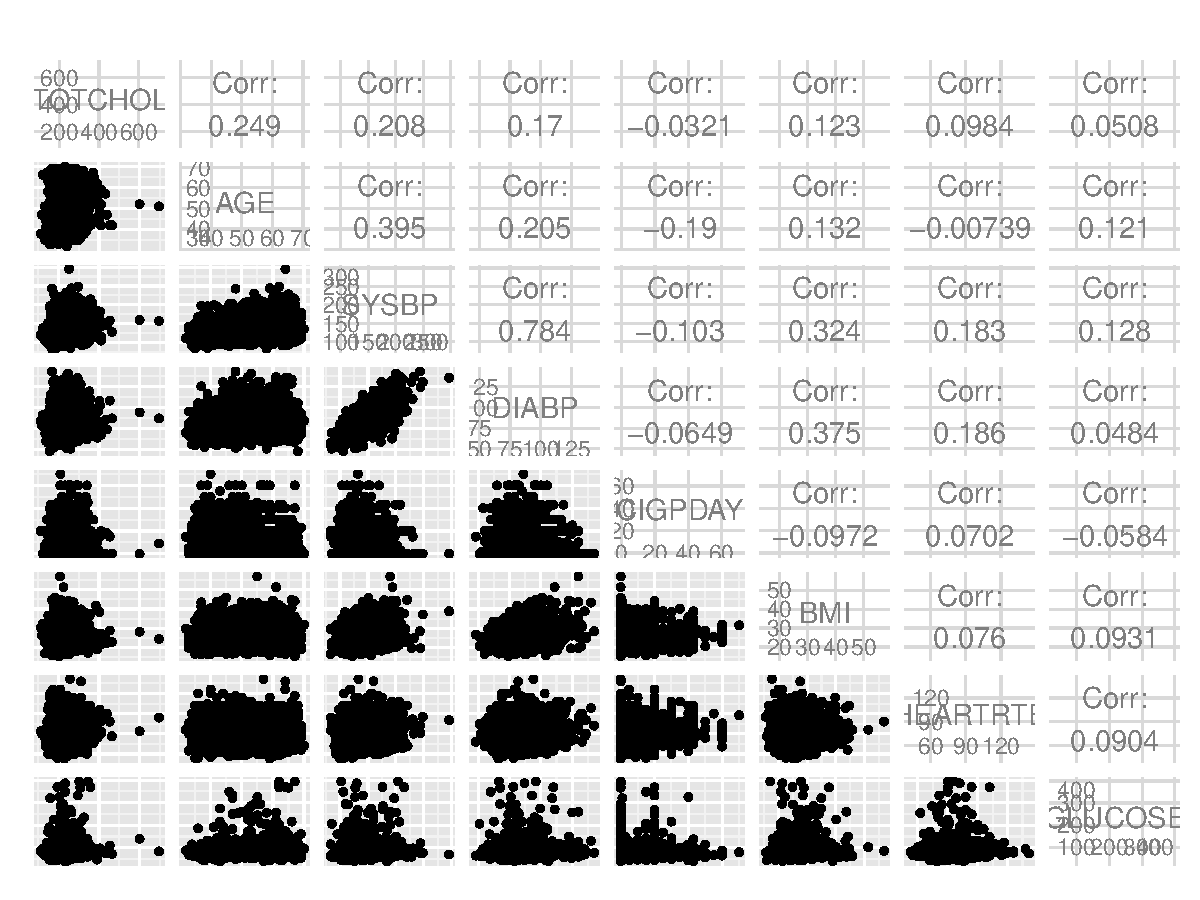
\includegraphics[width=1\textwidth]{Rplot.pdf}
    \caption{Awesome Image}
    \label{fig:awesome_image}
\end{center}
\end{figure}
\newpage

From the figure we can see that the most consistent correlation between one variable and the others seems to be Systolic Blood pressure.  This is a good outcome variable because it intuitively makes sense as an outcome, whereas other variables such as BMI occur in a large part due to environmental factors that aren't factored into this study such as diet. Originally, I was thinking of using Total Cholestrol, however it has relatively weak correlation with many of the factors of interest. Systolic Blood Pressure has the strongest correlation with Diabolic Blood Pressure, however this is a relatively uninteresting relationship to study as it they can be considered more or less colinear. We can move on instead to the next highest correlation which is BMI.
\subsection{Simple Liinear Regression Analysis}
\begin{Schunk}
\begin{Sinput}
> m1<-lm(SYSBP~BMI, data=frm2)
> summary(m1)
\end{Sinput}
\begin{Soutput}
Call:
lm(formula = SYSBP ~ BMI, data = frm2)

Residuals:
    Min      1Q  Median      3Q     Max 
-56.214 -14.776  -3.833  10.422 138.903 

Coefficients:
            Estimate Std. Error t value Pr(>|t|)    
(Intercept) 86.66684    2.02861   42.72   <2e-16 ***
BMI          1.78852    0.07752   23.07   <2e-16 ***
---
Signif. codes:  0 '***' 0.001 '**' 0.01 '*' 0.05 '.' 0.1 ' ' 1

Residual standard error: 21.12 on 4413 degrees of freedom
  (19 observations deleted due to missingness)
Multiple R-squared:  0.1076,	Adjusted R-squared:  0.1074 
F-statistic: 532.3 on 1 and 4413 DF,  p-value: < 2.2e-16
\end{Soutput}
\begin{Sinput}
> qplot(BMI, SYSBP, data=frm2) + geom_smooth(method="lm",se=TRUE)
\end{Sinput}
\end{Schunk}
From our simple linear modeling summary we can see a conclude that there is an association between systolic blood pressure and BMI.  The adjusted $R^2$ is relatively low.  It would be interesting to see then the effect of adding new variables to our model.

\begin{Schunk}
\begin{Sinput}
> # Convert data type of SEX variable from integer to factor 
> frm1_du <- frm1
> frm1_du$SEX <- as.factor(frm1_du$SEX)
> # Multiple regression model, 1 continuous and 1 categorical variables
> m2<-lm(SYSBP~BMI+factor(SEX), data=frm1_du)
> summary(m2)
\end{Sinput}
\begin{Soutput}
Call:
lm(formula = SYSBP ~ BMI + factor(SEX), data = frm1_du)

Residuals:
    Min      1Q  Median      3Q     Max 
-54.537 -14.673  -3.649  10.695 137.161 

Coefficients:
             Estimate Std. Error t value Pr(>|t|)    
(Intercept)   84.1945     2.0838  40.404  < 2e-16 ***
BMI            1.8153     0.0775  23.423  < 2e-16 ***
factor(SEX)2   3.1734     0.6405   4.955 7.51e-07 ***
---
Signif. codes:  0 '***' 0.001 '**' 0.01 '*' 0.05 '.' 0.1 ' ' 1

Residual standard error: 21.07 on 4412 degrees of freedom
  (19 observations deleted due to missingness)
Multiple R-squared:  0.1126,	Adjusted R-squared:  0.1122 
F-statistic: 279.9 on 2 and 4412 DF,  p-value: < 2.2e-16
\end{Soutput}
\begin{Sinput}
> qplot(BMI, SYSBP, data=frm1_du, color=SEX) + geom_smooth(method="lm",se=TRUE)
> # Another trial with another continuous variable
> m3<-lm(SYSBP~AGE+factor(SEX), data=frm1_du)
> summary(m3)
\end{Sinput}
\begin{Soutput}
Call:
lm(formula = SYSBP ~ AGE + factor(SEX), data = frm1_du)

Residuals:
    Min      1Q  Median      3Q     Max 
-56.682 -13.786  -2.646  10.426 146.818 

Coefficients:
             Estimate Std. Error t value Pr(>|t|)    
(Intercept)  80.54502    1.83136  43.981  < 2e-16 ***
AGE           1.02823    0.03557  28.905  < 2e-16 ***
factor(SEX)2  1.82999    0.62199   2.942  0.00328 ** 
---
Signif. codes:  0 '***' 0.001 '**' 0.01 '*' 0.05 '.' 0.1 ' ' 1

Residual standard error: 20.55 on 4431 degrees of freedom
Multiple R-squared:  0.1604,	Adjusted R-squared:  0.1601 
F-statistic: 423.4 on 2 and 4431 DF,  p-value: < 2.2e-16
\end{Soutput}
\begin{Sinput}
> qplot(AGE, SYSBP, data=frm1_du, color=SEX) + geom_smooth(method="lm",se=TRUE)
> # Another trial with another continuous variable
> m4<-lm(GLUCOSE~AGE+factor(SEX), data=frm1_du)
> summary(m4)
\end{Sinput}
\begin{Soutput}
Call:
lm(formula = GLUCOSE ~ AGE + factor(SEX), data = frm1_du)

Residuals:
    Min      1Q  Median      3Q     Max 
-44.486 -10.738  -3.690   5.019 307.438 

Coefficients:
             Estimate Std. Error t value Pr(>|t|)    
(Intercept)  64.89016    2.25723  28.748  < 2e-16 ***
AGE           0.34955    0.04381   7.979 1.91e-15 ***
factor(SEX)2 -0.32851    0.76586  -0.429    0.668    
---
Signif. codes:  0 '***' 0.001 '**' 0.01 '*' 0.05 '.' 0.1 ' ' 1

Residual standard error: 24.21 on 4034 degrees of freedom
  (397 observations deleted due to missingness)
Multiple R-squared:  0.01556,	Adjusted R-squared:  0.01507 
F-statistic: 31.88 on 2 and 4034 DF,  p-value: 1.828e-14
\end{Soutput}
\begin{Sinput}
> qplot(AGE, GLUCOSE, data=frm1_du, color=SEX) + geom_smooth(method="lm",se=TRUE)
> 
\end{Sinput}
\end{Schunk}

\end{document}
